% !TeX document-id = {7b7d88a4-0972-4202-9c89-33327d1050f5}
% !TeX spellcheck = en_EN
\documentclass[10pt, dvipsnames]{beamer}
\usepackage{appendixnumberbeamer}
\usepackage[T1]{fontenc}
\usepackage[utf8]{inputenc}
\usepackage{hyperref}
\usepackage{fontawesome5, lipsum}
\usepackage{graphicx}
\usepackage[USenglish]{babel}
\usepackage{setspace, multicol, makecell, booktabs, multirow}
\usepackage{mathtools, amsthm, amsfonts, siunitx, physics, chemformula, empheq}
\usepackage{mtpro2, pifont, custom}
\pdfmapfile{=mtpro2.map}
\usepackage[backend=biber, abbreviate=true, doi=false, style=numeric-comp, giveninits=true, sorting=none]{biblatex}
\usepackage{enumitem, csquotes, xurl}
\usepackage[most]{tcolorbox}
\usepackage{multimedia, tikz}
\usepackage[font=footnotesize, bf, format=plain, font=normalsize]{caption}

\usetikzlibrary{math}

\graphicspath{ {./bilder/} }
\addbibresource{literatur.bib}

%\catcode`_=\active
%\newcommand_[1]{\ensuremath{\sb{\fontfamily{Times New Roman}\selectfont \mathrm{#1}}}}

\AtBeginDocument{\sisetup{per-mode = symbol, sticky-per, mode=text, text-font-command=\fontfamily{Times New Roman}\selectfont}}
\let\oldunit\unit
\renewcommand{\unit}[1]{\hspace{4pt}\oldunit{#1}}
\DeclareSIUnit\year{yr}

\newcommand{\nair}{n\sb{\fontfamily{Times New Roman}\selectfont \mathrm{air}}}

\usepackage{scalerel,stackengine}
\newcommand\equalhat{\mathrel{\stackon[1.5pt]{=}{\stretchto{%
				\scalerel*[\widthof{=}]{\wedge}{\rule{1ex}{3ex}}}{0.5ex}}}}

% ------------------------------------------------------------------------------
% Use the beautiful metropolis beamer template
% ------------------------------------------------------------------------------
%\usepackage{FiraSans} 
\mode<presentation>
{
	\usetheme[progressbar=frametitle,background=light]{metropolis} 
	\usecolortheme{default} % or try albatross, beaver, crane, ...
	\usefonttheme[onlymath]{serif}  % or try serif, structurebold, ...
	\setbeamertemplate{navigation symbols}{}
	\setbeamertemplate{caption}[numbered]
	\setbeamertemplate{section in toc}[sections numbered]
	\setbeamerfont{frametitle}{size=\LARGE}
	\metroset{block=fill}
} 

\makeatletter
\setlength{\metropolis@progressinheadfoot@linewidth}{3pt}
\setlength{\metropolis@titleseparator@linewidth}{3pt}
\setlength{\metropolis@progressonsectionpage@linewidth}{3pt}

\makeatother

% ------------------------------------------------------------------------------
% tcolorbox / tcblisting
% ------------------------------------------------------------------------------	
\definecolor{MyBlue}{HTML}{0072B2}
\definecolor{MyOrange}{HTML}{D55E00}
\definecolor{MyRed}{HTML}{F00F0F}

\setstretch{1.5}

\newtcolorbox{quotebox}{enhanced, colframe=MyOrange, top=0.2cm, bottom=0.2cm, colback=orange!15, left=0.1cm}

\title{Das Hubble Gesetz}
\author{Alexander Helbok}
\date{\today}

\begin{document}
	\maketitle
%	\begin{frame}[noframenumbering, plain]{Overview}
%		\tableofcontents
%	\end{frame}

	\begin{frame}{Timeline}
		\begin{tikzpicture}[scale=2, every node/.style={scale=0.8, black}]
			\draw[line width=1.5pt] (0, 0) -- (5, 0);
			\foreach \i in {0,...,5}{
			\draw[MyBlue, fill](\i,0) circle (.045) node [below, yshift=-0.2cm] {\Large\( 19\i0 \)};}
			
			\draw[MyBlue, line width=1pt] (0.5, 0) -- (0.5, 0.25) node [above left, xshift=0.5cm] {SRT (1905)};
			
			\draw[MyBlue, line width=1pt] (1.5, 0) -- (1.5, .75) node [above left, xshift=0.2cm] {ART (1915)};
			
			\draw[MyBlue, line width=1pt] (1.7, 0) -- (1.7, 1.25) node [above left, align=left] {Einstein/de Sitter\\ Universum (1917)};
			
			\draw[MyBlue, line width=1pt] (1.9, 0) -- (1.9, 2) node [above left, align=left] {Eddington: Beweis über\\ Lichtumlenkung (1919)};
			
			\draw[MyBlue, line width=1pt] (2.2, 0) -- (2.2, 2.5) node [above right, xshift=-0.4cm] {Friedmann's Gleichungen (1922)};
			
			\draw[MyBlue, line width=1pt] (2.7, 0) -- (2.7, 1.5) node [above right, align=left, xshift=-0.4cm] {Lema\^{i}tres expandierendes\\ Universum (1927)};
			
			\draw[MyOrange, line width=1pt] (2.9, 0) -- (2.9, 0.8) node [above right, align=left, xshift=-0.5cm] {Hubble Messungen\\ (1929, 1931, 1934)};
			\draw[MyOrange, line width=1pt] (3.1, 0) -- (3.1, 0.8);
			\draw[MyOrange, line width=1pt] (3.4, 0) -- (3.4, 0.8);
			
			\draw[MyRed, line width=1pt] (4.8, 0) -- (4.8, 0.5) node [above] {CMBR postuliert (1948)};
		\end{tikzpicture}
	\end{frame}

	\begin{frame}{\( 100- \)Zoll Hooker Teleskop}
		\begin{tikzpicture}
			\node[anchor=south west,inner sep=0] (image) at (0,0) {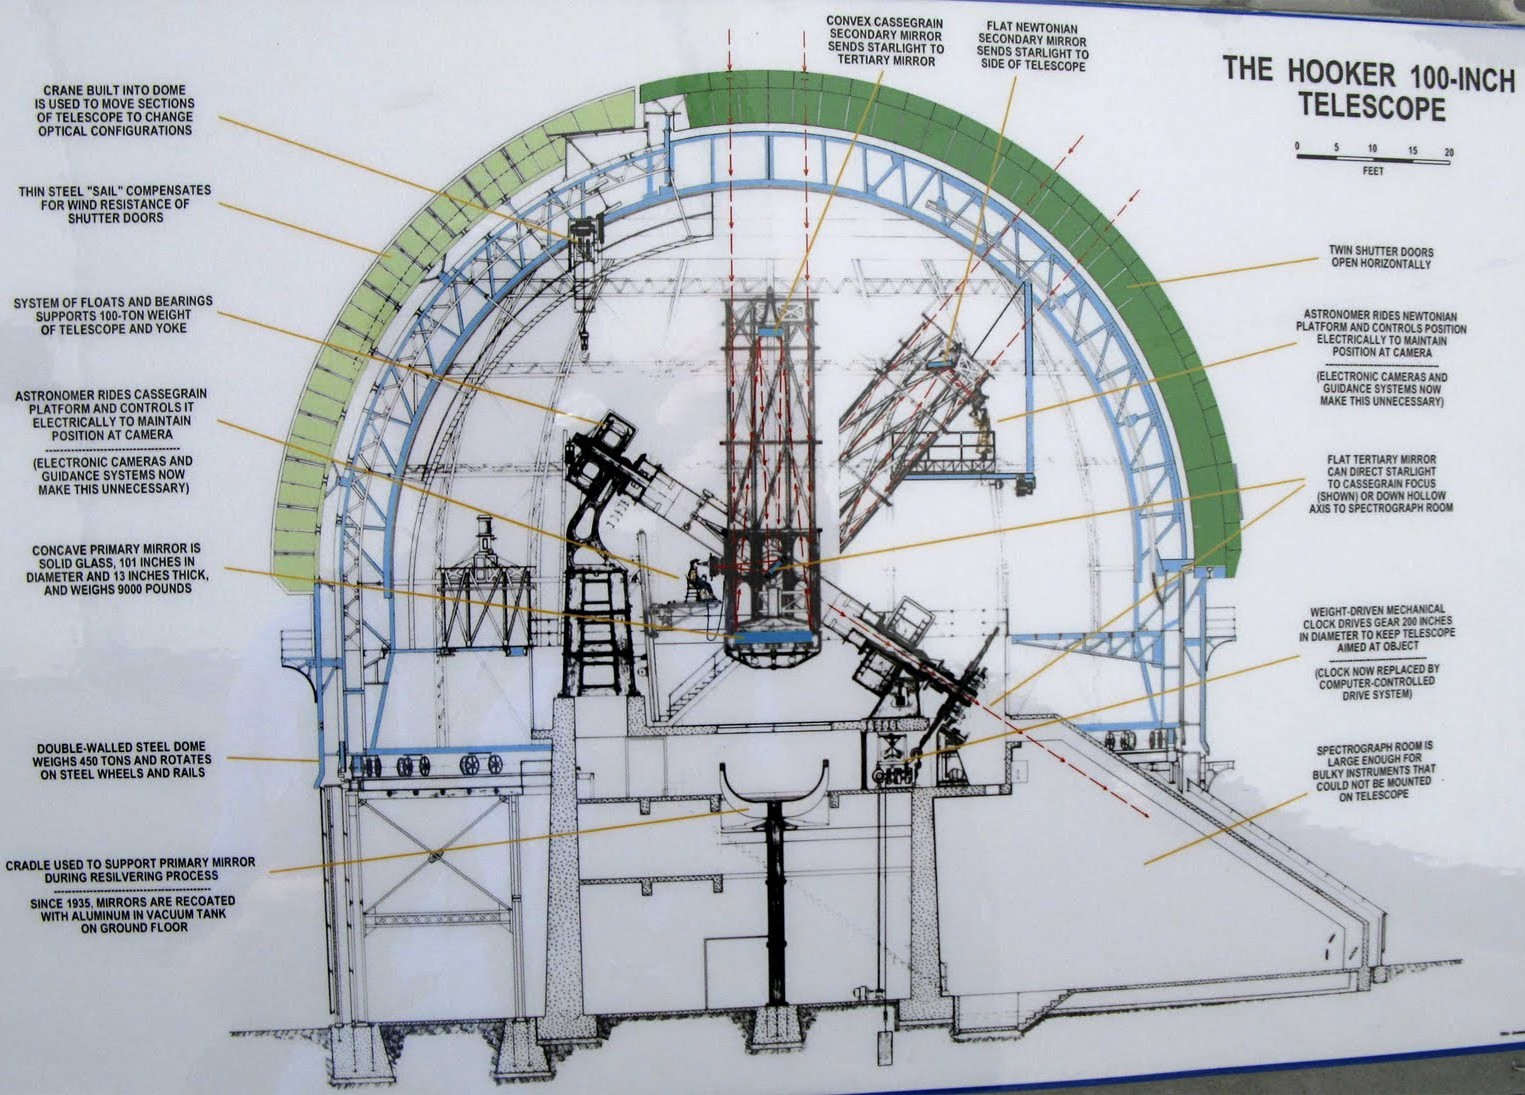
\includegraphics[width=\textwidth]{Hooker2}};
			\begin{scope}[x={(image.south east)},y={(image.north west)}]
				\node[] at (0.21, 0.975) {\tiny\citetitle{Hooker} \cite{Hooker}};
			\end{scope}
		\end{tikzpicture}
	\end{frame}
	
%	########### Theorie #############
	\begin{frame}{Enternungsbestimmung der Nebulae}
		Geschwindigkeit von 46 Nebel von Slipher vermessen (Doppler-shift) \cite{slipher1915spectrographic} \\
		Enfernungsbestimmung von Hubble über
		\begin{itemize}[label={\textendash}, itemindent=0.5cm]
			\item Cepheiden Perioden-Leuchtkraft-Beziehung (7)
			\item Vergleich mit bekannten Galaxien (13)
			\item statistische Leuchtkraftverteilung von Nebel (4)
		\end{itemize}
	\end{frame}
	
	\begin{frame}{Analyse}
		\[ v = rK + \tikzmark{1} X\cos(\delta)\cos(\alpha) + Y\cos(\delta)\sin(\alpha) + Z\sin(\delta) \tikzmark{2} \]\\[4ex]
		
		\begin{quotebox}\hspace{0.1cm} \blockcquote{Hubble1929}{Two solutions have been made, ...}\end{quotebox}
		
		\begin{tikzpicture}
			\node[anchor=south west,inner sep=0] (image) at (0,0) {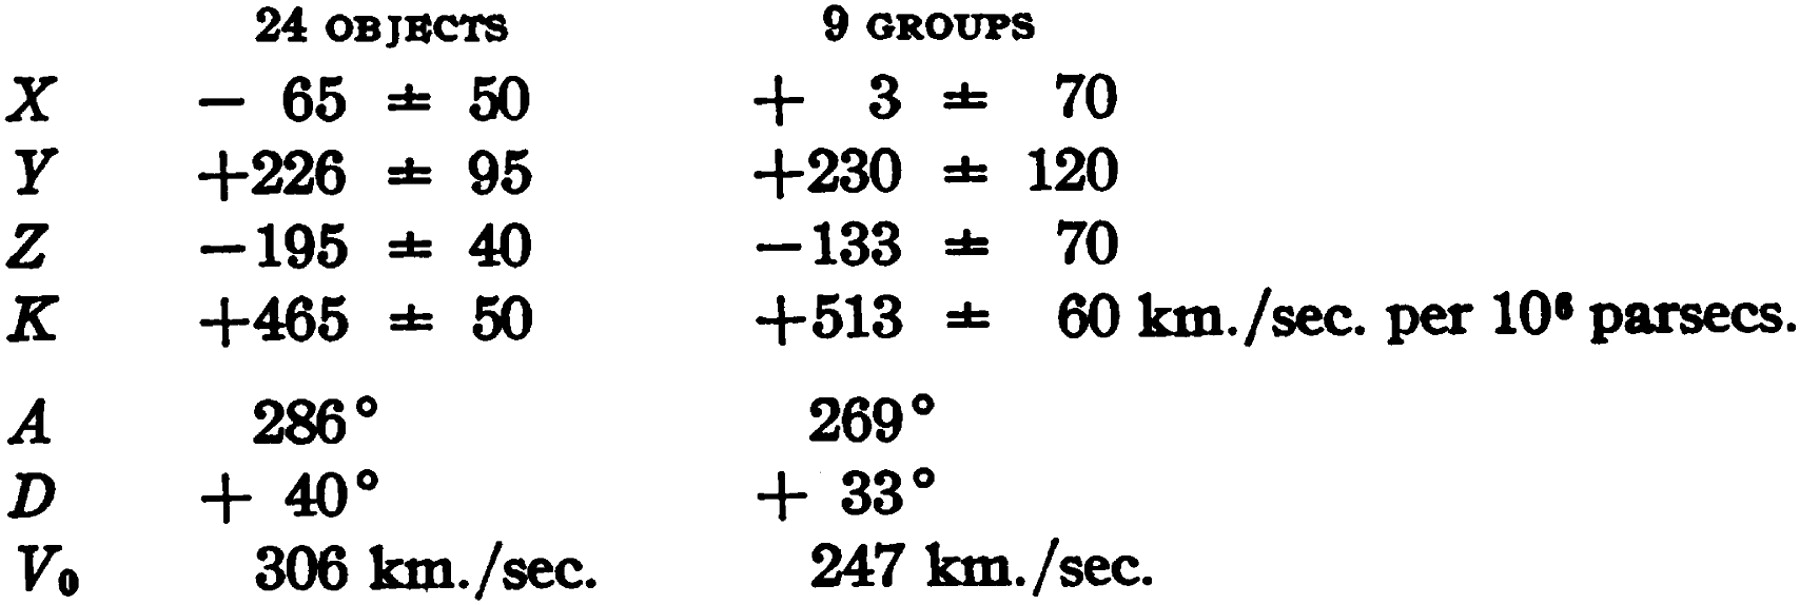
\includegraphics[width=\textwidth]{solutions}};
			\begin{scope}[x={(image.south east)},y={(image.north west)}]
				\node[] at (0.9, 0.05) {(\citeauthor{Hubble1929} \citeyear{Hubble1929})};
			\end{scope}
		\end{tikzpicture}
		\AddUnderBrace[0.15]{1}{2}{Relativgeschwindigkeit \( V_0 \)}
	\end{frame}
	
%	########## ergebnisse ##########
	\begin{frame}{Ergebnisse}
		\begin{tikzpicture}
			\begin{scope}[xshift=1.5cm]
				\node[anchor=south west,inner sep=0] (image) at (0,0) {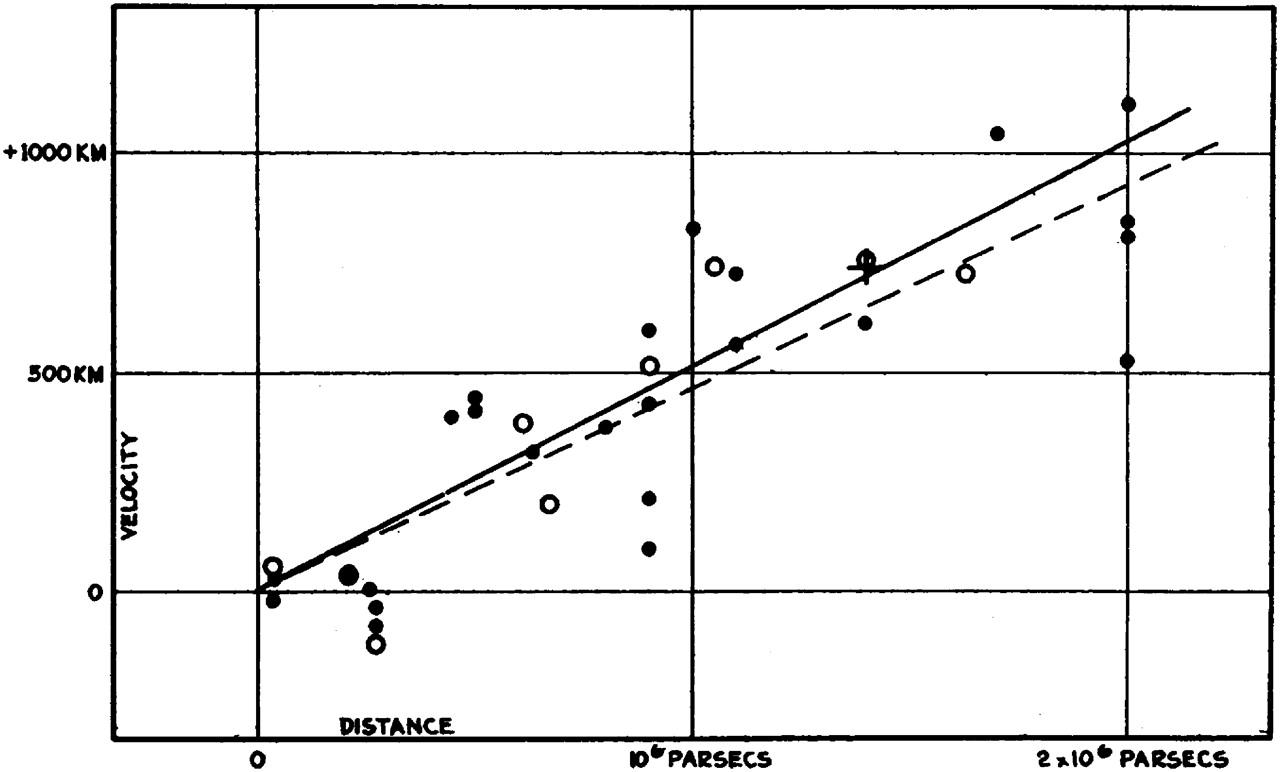
\includegraphics[width=\textwidth]{HubbleLaw}};
				\begin{scope}[x={(image.south east)},y={(image.north west)}]
					\begin{onlyenv}<1>
						\fill[Gray, opacity=0.3, rounded corners] (0.205, 0.665) rectangle (0.5, 0.97);
						\draw[MyOrange,ultra thick,rounded corners] (0.2,0.15) rectangle (0.31,0.3);
						\draw[MyOrange,ultra thick,rounded corners] (0.335,0.43) rectangle (0.37,0.49);
						
						\draw[rotate around={-60:(0.575,0.55)},MyBlue, ultra thick] (0.575,0.55) ellipse (40pt and 95pt);
	%					\draw[red, ultra thick, line cap=round] (0.345,0.445) -- (0.36,0.475);
	%					\draw[red, ultra thick, line cap=round] (0.345,0.475) -- (0.36,0.445);
						
						\draw[MyRed,ultra thick,rounded corners] (0.86,0.5) rectangle (0.9,0.9);
						
%						Legend
						\begin{scope}[shift={(-0.48, 0.6)}]							
							\draw[MyOrange,ultra thick,rounded corners] (0.7,0.3) rectangle (0.73,0.35) node [black, right, yshift=-0.18cm] {Cepheiden};
							\draw[MyBlue,ultra thick,rounded corners] (0.7,0.22) rectangle (0.73,0.27) node [black, right, yshift=-0.18cm] {Standardkerzen};
							\draw[MyRed,ultra thick,rounded corners] (0.7,0.14) rectangle (0.73,0.19) node [black, right, yshift=-0.18cm] {Virgo};
							\draw[ultra thick, line cap=round] (0.7, 0.1) -- (0.73, 0.1) node [right] {Fit};
						\end{scope}
					\end{onlyenv}
					\begin{onlyenv}<2>
						\fill[Gray, opacity=0.3, rounded corners] (0.205, 0.72) rectangle (0.5, 0.89);
%						Legend
						\begin{scope}[shift={(-0.48, 0.6)}]
							\draw[line width=1.25pt] (0.715,0.24) circle (2 pt) node [right, xshift=0.18cm] {Gebinnte Daten};
							\draw[ultra thick, line cap=round, dashed] (0.7, 0.16) -- (0.73, 0.16) node [right] {Fit};
						\end{scope}
					\end{onlyenv}
					\begin{onlyenv}<3>
						\fill[Gray, opacity=0.3, rounded corners] (0.205, 0.805) rectangle (0.55, 0.88);
						\draw[MyRed,ultra thick, rounded corners] (0.65,0.62) rectangle (0.7,0.69);
%						Legend
						\begin{scope}[shift={(-0.48, 0.6)}]
							\draw[line width=1.25pt, line cap=round] (0.7, 0.24) -- (0.73, 0.24) node [right, xshift=0.05cm] {Gemittelte Daten};
							\draw[line width=1.25pt, line cap=round] (0.715, 0.22) -- (0.715, 0.26);
						\end{scope}
					\end{onlyenv}
					
					\node[] at (0.9, -0.05) {(\citeauthor{Hubble1929} \citeyear{Hubble1929})};
%					\foreach \i in {1,...,10}{
%					\draw[black] (0.\i, 0) -- (0.\i, 1);
%					\draw[black] (0, 0.\i) -- (1, 0.\i);}
				\end{scope}
			\end{scope}
		\end{tikzpicture}
	\end{frame}
	
%	######### 1st Interpretation ########
	\begin{frame}{Intrepretation von Hubble}
		\vspace{0.5cm}
		\begin{minipage}[b][.425\textheight][t]{\textwidth}
		\begin{quotebox}
			\begin{itemize}
				\only<1>{\item[1)] \blockcquote{Hubble1929}{The results establish a roughly linear relation between velocities and distances among nebulae ...}\\
				Mit Faktor \( K = 465(50) \text{ bzw. } 513(60) \unit{km/s/Mpc} \)}
				\only<2>{\item[2)] \blockcquote{Hubble1929}{New data to be expected in the near future may modify the significance of the present investigation or, if confirmatory, will lead to a solution having many times the weight.}}
				\only<3>{\item[3)] \blockcquote{Hubble1929}{The outstanding feature, however, is the possibility that the velocity-distance relation may represent the de Sitter effect, ...}}
			\end{itemize}
		\end{quotebox}
	\end{minipage}
	\begin{minipage}[b][.5\textheight][t]{\textwidth}
			\begin{itemize}[label={\textendash}]
				\only<1>{
					\item linearer Zusammenhang deutlich sichtbar
					\item keine statistischen Fehler
					\item dafür Entfernungen systematisch zu klein (Faktor 7!)
					\item keine Fitgüte im Paper}
				\only<2>{
					\item Absolut Richtig
					\item viele Nachfolgeexperimente (bis heute noch)
					\item "crisis in cosmology"}
				\only<3>{
					\item deSitter Universum: statisch, keine Materie
					\item Redshift durch Zeitverlangsamung bei großen Entfernungen \cite{deSitter}
					\item Y}
			\end{itemize}
		\end{minipage}
	\end{frame}
	
%	######### folgeexperimente #########
	\begin{frame}{Typ1a Supernovae}
		Theorie und leuchtkraftrelation
	\end{frame}

	\begin{frame}{Messung über SN1a}
		\centering
		\begin{tikzpicture}
			\node[anchor=south west,inner sep=0] (image) at (0,0) {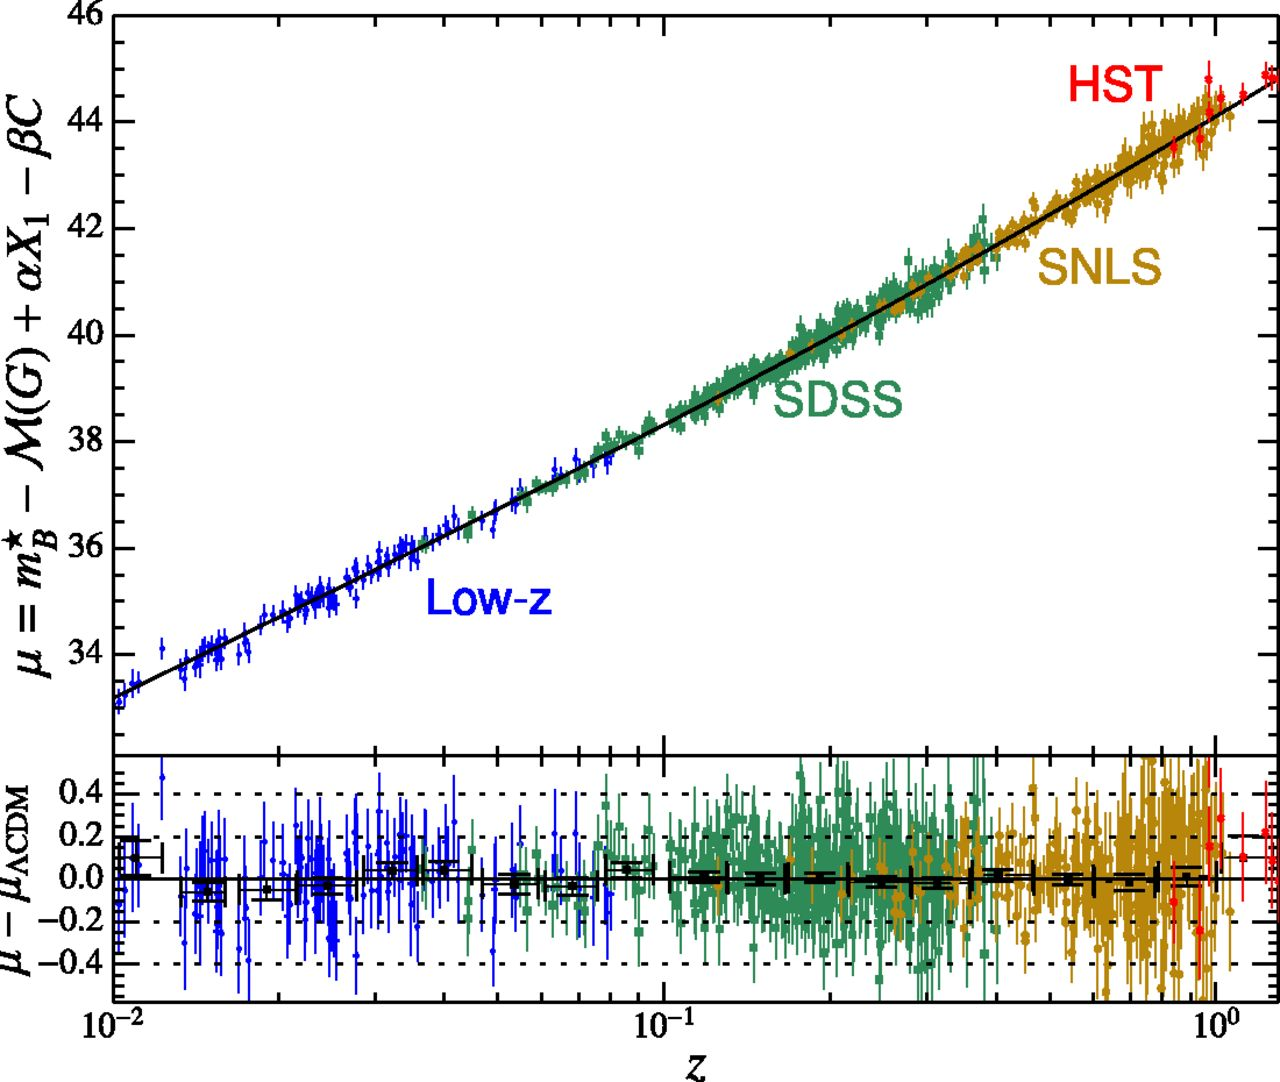
\includegraphics[height=0.9\textheight]{Sn1a}};	
			
			\begin{scope}[x={(image.south east)},y={(image.north west)}]

				\only<1>{\draw[line width=1pt, opacity=0] (0.09, 0.355) -- (1, 0.89);}
				\only<2>{\draw[line width=1pt] (0.09, 0.355) -- (1, 0.89);}
				\node[] at (0.75, 0.02) {(\citeauthor{betoule2014improved} \citeyear{betoule2014improved})};
%				\draw[fill] (0.5, 0.59) circle (.005) node [below] {\( \approx 1.4 \unit{\giga\year} \)};
			\end{scope}
		\end{tikzpicture}
	\end{frame}
	
	\begin{frame}{Krise}
		\begin{tikzpicture}
			\node[anchor=south west,inner sep=0] (image) at (0,0) {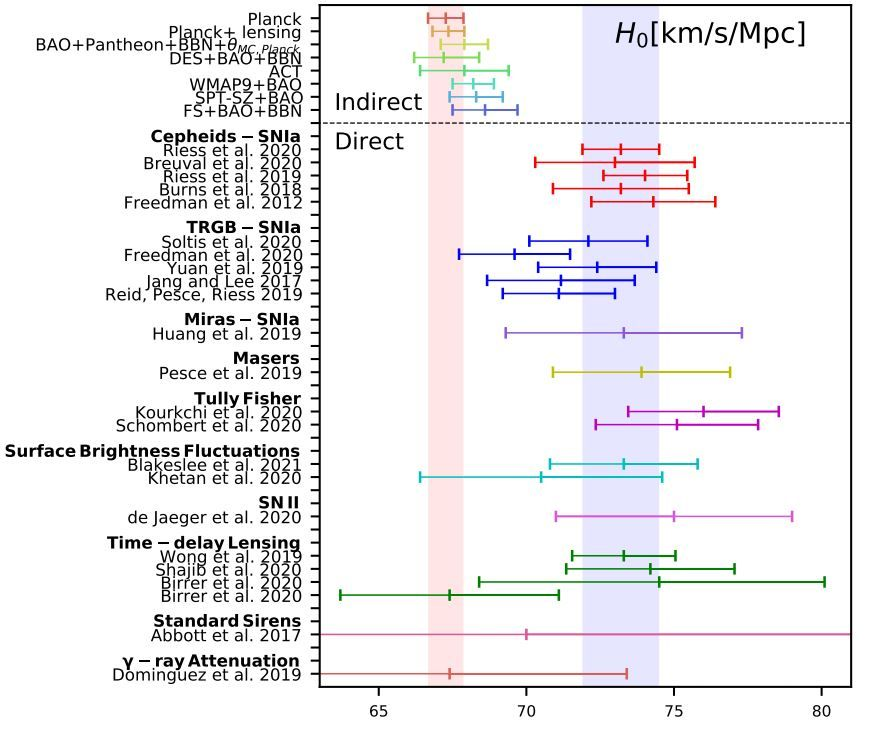
\includegraphics[height=0.9\textheight]{crisis}};
			
			\begin{scope}[x={(image.south east)},y={(image.north west)}]
				\node[] at (0.15, 0.02) {(\citeauthor{Di_Valentino_2021} \citeyear{Di_Valentino_2021})};
			\end{scope}
		\end{tikzpicture}
	\end{frame}
%	######### Interpretation

% 	######### Recap #########
	\begin{frame}{Recap}
		\begin{itemize}[label={\textendash}, itemindent=0.1cm]
			\item Entferungsbestimmung von Nebeln über verschiedene Leuchtkraftrelationen
			\item Geschwindigkeit über Doppler shift
			\item[\( \Rightarrow \)] Linearer Zusammenhang (obwohl systematische Abweichung)
			\item 
		\end{itemize}
	\end{frame}

\begin{frame}[standout]
	\Huge Fragen?
\end{frame}

\appendix

\begin{frame}{Frage 1}
%	Wäre Hubble zum gleichen Schluss gekommen, wären die Fehler statistisch und nicht systematisch?	
	Wenn jetzt alle Galaxien von uns wegfliegen, heißt das, dass wir uns im Zentrum des Universums befinden wo der Urknall stattfand?
	\begin{itemize}
		\item[A)] Ja, weil ... 
		\item[B)] Nein, weil ...
	\end{itemize}
\end{frame}

\begin{frame}{Frage 2}
	Warum habe ich \( H_0 \) immer Hubble Parameter und nicht Hubble Konstante (wie man es in vielen Lehrbüchern und sieht) genannt?
	\begin{itemize}
		\item[A)] Die beiden Begriffe sind ja Synonyme
		\only<1>{\item[B)] Naja, \( H_0 \) ist ja zeitlich nicht konstant geblieben}
		\only<2>{{\color{Green}\item[B)] Naja, \( H_0 \) ist ja zeitlich nicht konstant geblieben}}
		\item[C)] Man kann \( H_0 \) nicht aus Naturkonstanten ableiten, also ist es selber keine Konstante
	\end{itemize}
\end{frame}

\begin{frame}{Backup/Theory slide}
	cepehid relation, SN1a relation
\end{frame}

\begin{frame}[allowframebreaks]{Sources}
	\printbibliography
\end{frame}

\end{document}